%%%%%%%%%%%%%%%%%%%%%%%%%%%%%%%%%%%%%%%%%
% Short Sectioned Assignment
% LaTeX Template
% Version 1.0 (5/5/12)
%
% This template has been downloaded from:
% http://www.LaTeXTemplates.com
%
% Original author:
% Frits Wenneker (http://www.howtotex.com)
%
% License:
% CC BY-NC-SA 3.0 (http://creativecommons.org/licenses/by-nc-sa/3.0/)
%
%%%%%%%%%%%%%%%%%%%%%%%%%%%%%%%%%%%%%%%%%

%----------------------------------------------------------------------------------------
%   PACKAGES AND OTHER DOCUMENT CONFIGURATIONS
%----------------------------------------------------------------------------------------

\documentclass[paper=letter, fontsize=11pt]{scrartcl} % A4 paper and 11pt font size
\synctex=1
\usepackage[T1]{fontenc} % Use 8-bit encoding that has 256 glyphs
\usepackage{fourier} % Use the Adobe Utopia font for the document - comment this line to return to the LaTeX default
\usepackage[english]{babel} % English language/hyphenation
\usepackage{amsmath,amsfonts,amsthm} % Math packages
%\usepackage[nolists, nomarkers]{endfloat}
\usepackage{hyperref}
\usepackage{bm}
\usepackage{graphicx}
\usepackage[section]{placeins}
\usepackage{sectsty} % Allows customizing section commands
\allsectionsfont{\normalfont\scshape} % Make all sections centered, the default font and small caps

\usepackage{fancyhdr} % Custom headers and footers
\pagestyle{fancyplain} % Makes all pages in the document conform to the custom headers and footers
\fancyhead{} % No page header - if you want one, create it in the same way as the footers below
\fancyfoot[L]{} % Empty left footer
\fancyfoot[C]{} % Empty center footer
\fancyfoot[R]{\thepage} % Page numbering for right footer
\renewcommand{\headrulewidth}{0pt} % Remove header underlines
\renewcommand{\footrulewidth}{0pt} % Remove footer underlines
\setlength{\headheight}{13.6pt} % Customize the height of the header

\numberwithin{equation}{section} % Number equations within sections (i.e. 1.1, 1.2, 2.1, 2.2 instead of 1, 2, 3, 4)
\numberwithin{figure}{section} % Number figures within sections (i.e. 1.1, 1.2, 2.1, 2.2 instead of 1, 2, 3, 4)
\numberwithin{table}{section} % Number tables within sections (i.e. 1.1, 1.2, 2.1, 2.2 instead of 1, 2, 3, 4)

\setlength\parindent{0pt} % Removes all indentation from paragraphs -
                          % comment this line for an assignment with
                          % lots of text
\setlength\parskip{12pt}


%----------------------------------------------------------------------------------------
%   TITLE SECTION
%----------------------------------------------------------------------------------------

\newcommand{\horrule}[1]{\rule{\linewidth}{#1}} % Create horizontal rule command with 1 argument of height

\title{ 
\normalfont \normalsize 
\textsc{Exoplanet Patchy Cloud Project} \\ [25pt] % Your university, school and/or department name(s)
\horrule{0.5pt} \\[0.4cm] % Thin top horizontal rule
\huge Cross Correlation Test and Preliminary Aperture Photometry Result\\ % The assignment title
\horrule{2pt} \\[0.5cm] % Thick bottom horizontal rule
}

\author{Yifan Zhou} % Your name

\date{\normalsize\today} % Today's date or a custom date

\begin{document}

\maketitle % Print the title
\section{Summary}
\begin{enumerate}
\item Cross Correlation method can align images with the saturated
  primary star centroid as precise as $\sim 0.01$ pixels, which is far
  better than the precision of IDL \texttt{cntrd.pro} or
  \texttt{gcntrd.pro} which is more than $\sim 0.2$ pixels. According
  to the residual image patterns, cross correlation alignment has
  better performance tan WCS alignment.
\item Aperture photometry for secondary object in ABPIC system is
  measured. The light curves are very similar to Glenn's
  measurement. However, the light curves for two filters, F125W and
  F160W agree with each other better in my measurement.
\item Considering only statistical uncertainties (counting errors) and
  fluctuation in the background, a rough estimate gives a result of
  0.3\% for relative uncertainty for one
  photometry measurement.
  
\end{enumerate}
\section{Image Alignment}
\subsection{Alignment Precision Test}
\subsection{The Modification for IDL \texttt{crosscorr} Routine}
\subsection{PSF subtraction result}
\begin{figure}
  \centering
  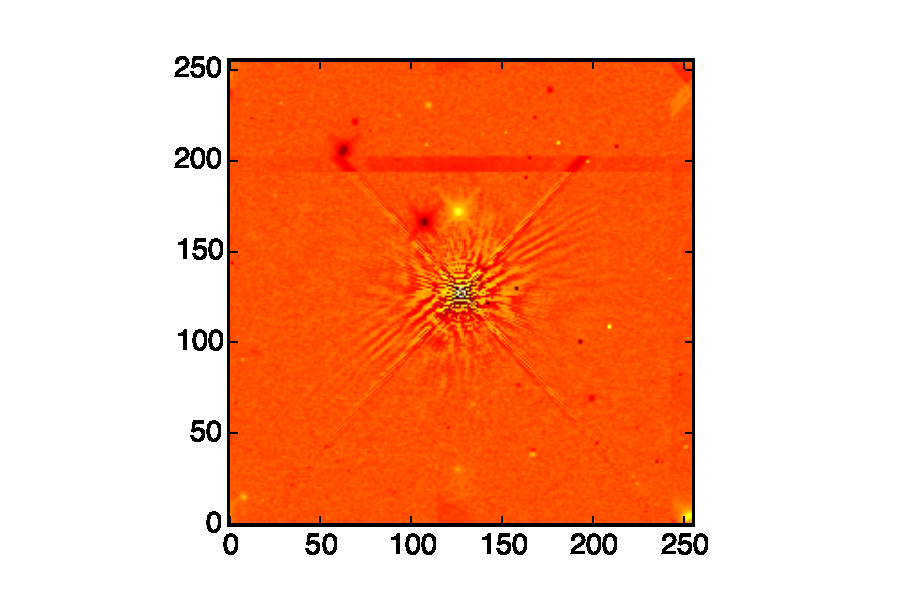
\includegraphics[width=\textwidth]{cc_example}
  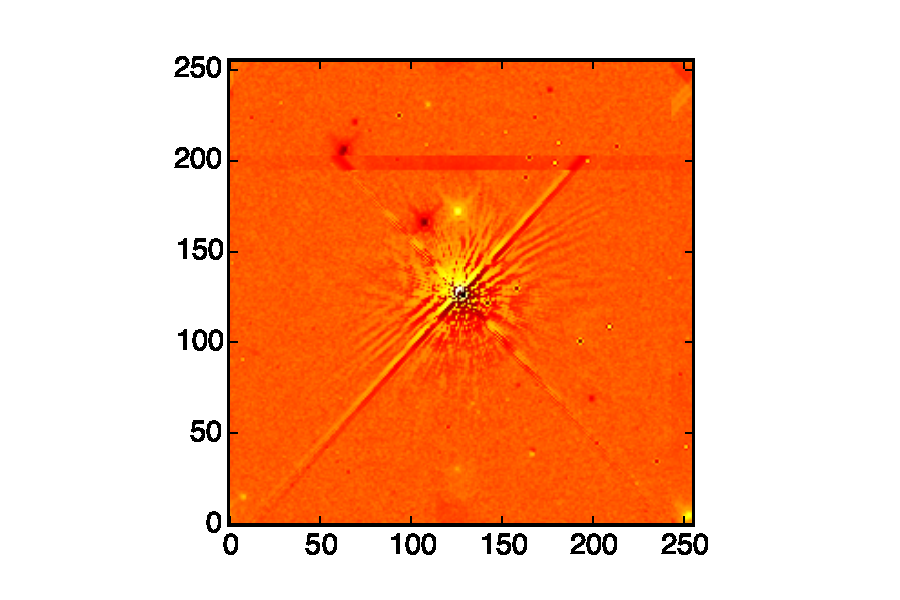
\includegraphics[width=\textwidth]{wcs_example}
  \caption{PSF subtraction comparison}\label{fig:subcomp}
\end{figure}
\section{Aperture Photometry Result}
\subsection{Light Curves}

The light curve measurements for both absolute fluxes and relative
fluxes are shown in Figure \ref{fig:lightcurve}. Figure
\ref{fig:glenn} is Glenn's preliminary measurements. The lower plot in
figure \ref{fig:lightcurve} is very similar to figure
\ref{fig:glenn}. However, in figure \ref{fig:glenn}, the light curves
for F125W and F160W show considerable discrepancies in 5th and 6th
orbits. However in my measurement, the two curves agree better. Apart
from this, the most prominent features are shown in both light
curves, e.g. the light curves are lower in 2nd orbit and the
discrepancy at start of the 3rd orbit.

\begin{figure}
  \centering
  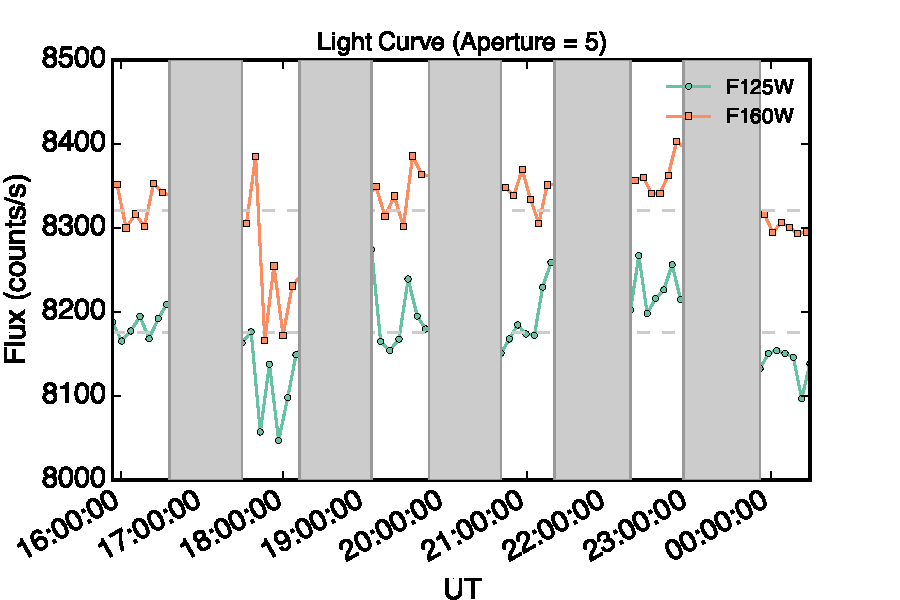
\includegraphics[width=0.8\textwidth]{fluxcurve_aper_05}
  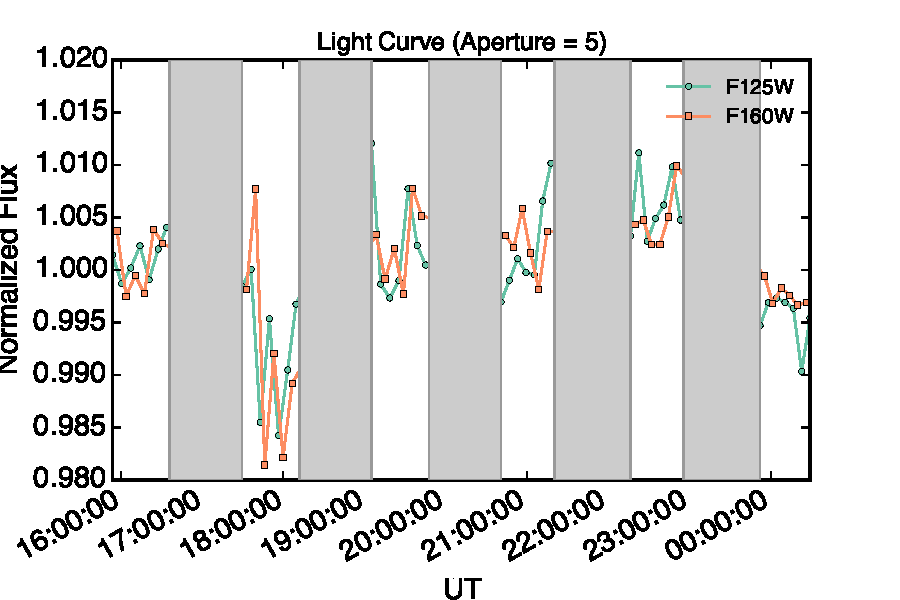
\includegraphics[width=0.8\textwidth]{relativefluxcurve_aper_05}
  \caption{Filter F125W and F160W light curves. Upper images shows the
    curve for absolute flux (count per second) changing with time. The
    mean values for both light curves are plotted with gray dashed
    lines. In the lower image, two light curves are normalized with
    the mean value of itself.}
  \label{fig:lightcurve}
\end{figure}

\begin{figure}
  \centering
    \centering
    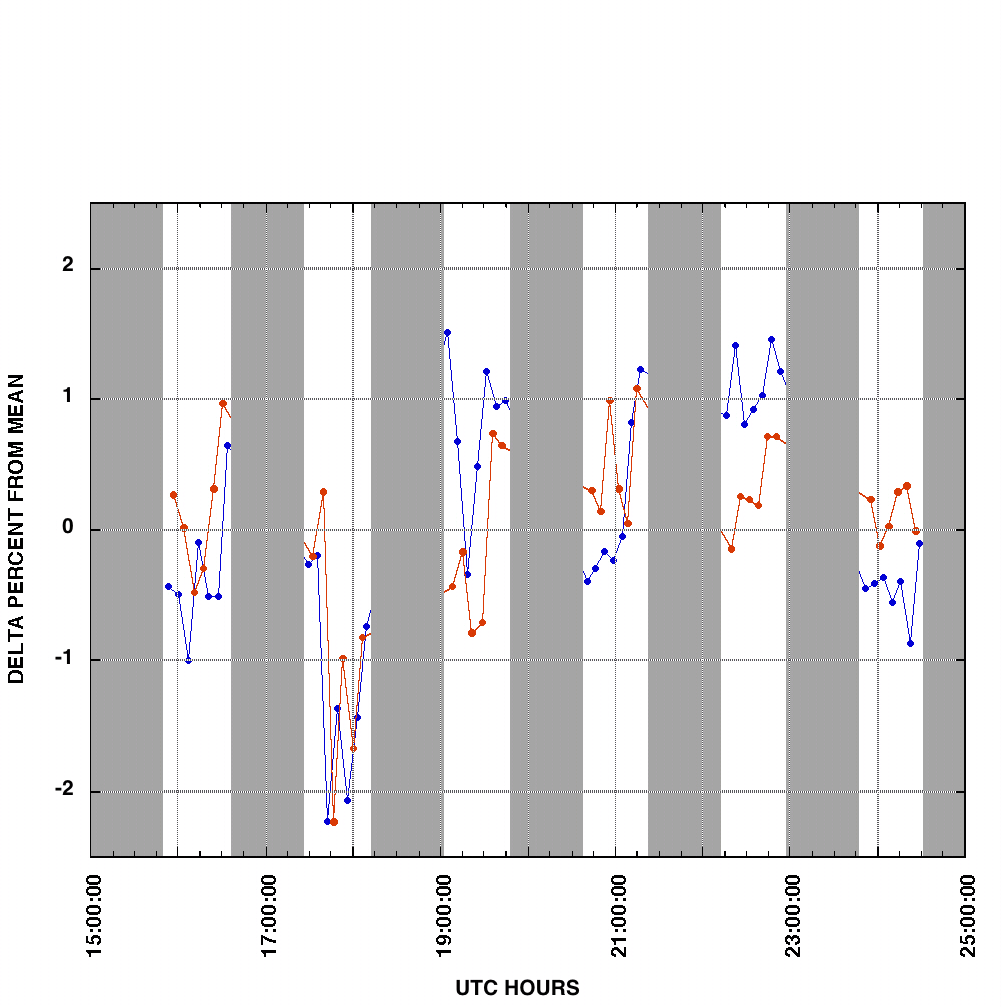
\includegraphics[width=0.8\textwidth]{ABPIC_DELTA_PERCENT_INITIAL}
    \caption{Glenn's preliminary measurement}
    \label{fig:glenn}
  \end{figure}

\subsection{Error Estimation}
Considering statistical uncertainty and fluctuation of background sky,
the relative error for one aperture photometry measurement is below
0.3\% according to my estimation. The error estimation procedure is
explained as following.\par

Statistical uncertainty:
\begin{equation}
  \sigma_{\mathrm{stat}}^{2}=ft_{\mathrm{expo}}
\end{equation}
Background fluctuation:
\begin{equation}
  \sigma_{\mathrm{sky}}^{2}=N\sigma_{\mathrm{sky,0}}^{2}t_{expo}
\end{equation}
Total error are the combination of these two parts:
\begin{equation}
  \sigma^{2} = \sigma_{\mathrm{stat}}^{2}+\sigma_{\mathrm{sky}}^{2}=ft_{\mathrm{expo}}+N\sigma_{\mathrm{sky,0}}^{2}t_{expo}
\end{equation}
Relative uncertainty:
\begin{equation}
  \frac{\sigma}{\mathrm{Flux}} = \frac{\sqrt{ft_{\mathrm{expo}}+N\sigma_{\mathrm{sky,0}}^{2}t_{expo}}}{ft_{\mathrm{expo}}}
\end{equation}
The exposure time are 30s for F125W images and 15s for F160W
images. Here I adopt 15s for a upper limit estimation. The flux
intensity for the exoplanet is $\sim 8000$ counts per second. The
standard deviation for background is $\sim 1$ counts per
second. Plugin those numbers, I estimated a relative uncertainty for 0.3\%.
\end{document}
%%% Local Variables:
%%% mode: latex
%%% TeX-master: t
%%% End:
